\chapter{Dinamica del punto materiale}
La dinamica è la branca della Fisica classica che si occupa di determinare perché un corpo si muove, a differenza della cinematica che descrive unicamente il moto senza occuparsi delle cause che lo hanno generato. L'intera dinamica si basa sui tre principi di Newton.
\begin{axiom}[principi di Newton]\hfill
    \begin{enumerate}
        \item Un corpo non soggetto a forze esterne, o tale che la risultante delle forze esterne agenti su di esso è pari a zero, permane nello stato di quiete o di moto rettilineo uniforme.
        \item La risultante delle forze applicate su un corpo è uguale in modulo al prodotto della massa del corpo per l'accelerazione, ed ha direzione e verso dell'accelerazione.
        \item Quando due corpi interagiscono, la forza che il primo corpo esercita sul secondo è uguale e opposta alla forza che il secondo esercita sul primo.
    \end{enumerate}
\end{axiom}
Secondo tali principi, la forza risultante è data da
\begin{equation}
    \vF=m\va=m\frac{d^2\vr}{dt^2},
\end{equation}
dove $m$ è la massa inerziale che rappresenta la tendenza di un corpo a preservare il proprio stato di quiete o di moto. 
\begin{defn}[sistema di riferimento]
    Un sistema di riferimento inerziale è un sistema che si muove di moto rettilineo uniforme rispetto a un altro e in cui vale il primo principio di Newton.
\end{defn}
\begin{obs}
    Un limite del secondo principio di Newton è che vale per velocità molto inferiori alla velocità della luce. Avvicinandosi a questo limite, gli effetti relativistici sono sempre meno trascurabili. 
\end{obs}
\begin{defn}[forza]
    La forza è la grandezza che esprime e misura l'interazione tra sistemi fisici.
\end{defn}
Nel caso di un moto uniformemente accelerato la risultante delle forze è diversa da zero. In particolare, agisce una forza costante $\vF$ e in generale la componente del moto parallela a $\vF$ è uniformemente accelerata con $\va=\vF/m$. Nelle altre direzioni ortogonali, non c'è moto se le componenti della velocità iniziale lungo tali direzioni sono nulle, oppure si ha un moto rettilineo uniforme se tali velocità sono diverse da zero.

Quando $\vF$ è variabile si ha un moto vario. In particolare, per il moto circolare si ha
\begin{equation}
    \vF=m\vaT+m\vaN=m\frac{dv}{dt}\huT+\frac{mv}{R^2}\huN=\vF_T+\vF_N.
\end{equation}
La risultante delle forze ha una componente ortogonale alla traiettoria $\vF_N$ che fa variare la direzione di $\vv$ e $\vF_T$ ne fa variare il modulo. 
La forza $\vF_N$ non è un tipo diverso di forza, ma è il nome che si dà alla componente ortogonale della risultante. 
\begin{defn}[quantità di moto]
    La quantità di moto (o il momento o l'impulso) di un corpo di massa $m$ che si muove di velocità $\vv$ è definita da 
    \begin{equation}
        \vp=m\vv.
    \end{equation}
\end{defn}
Dalla definizione di quantità di moto è immediato ricavare, se la massa $m$ è costante, che
\begin{equation}
    \vF=\frac{d\vp}{dt}.
\end{equation}
Quindi, l'azione di una forza $\vF$ in un tempo $dt$ produce una variazione $d\vp$ della quantità di moto. 
\begin{teo}[teorema dell'impulso]
    L'impulso di una forza che si esercita su un punto materiale in un intervallo di tempo è uguale alla variazione della quantità di moto del punto in quell'intervallo di tempo. L'impulso $J$ di tale forza è
    \begin{equation}
        J=\int_0^t\vF\,dt=\int_{\vp_0}^{\vp}d\vp=\vp-\vp_0=\Delta\vp.
    \end{equation}
\end{teo}
Da questo teorema si ricava immediatamente che
\begin{equation}
    \vF\Delta t=\Delta\vp.
\end{equation}
Quindi, la variazione dell'impulso $\Delta\vp$ è proporzionale all'intervallo di tempo $\Delta t$ in cui agisce la forza $\vF$. Quando $\vF=0$, allora $\Delta\vp=0$ e l'impulso è costante, ovvero si conserva.
\begin{ex}
    Come primo esempio di applicazione dei principi di Newton, si considerino due corpi di massa $m_1$ e $m_2$ posti a contatto su un piano orizzontale. Su ciascuno dei due corpi agisce una forza peso, $\vN_1=m_1\vg$ e $\vN_2=m_2\vg$ rispettivamente. Si supponga ora di applicare una forza $\vF$ sul corpo di massa $m_1$. Di conseguenza, sul secondo corpo agisce una forza $\vF_{1,2}$ indotta dal primo e, per il terzo principio di Newton, sul primo corpo agisce una forza uguale e opposta $\vF_{2,1}$. Calcolando la risultante delle forze per ciascun corpo si ottengono
\begin{equation}
    \begin{cases}
        F-F_{2,1}=m_1a_1 \\
        F_{1,2}=m_2a_2.
    \end{cases}
\end{equation}
Chiaramente, essendo i corpi a contatto, la loro accelerazione è la stessa, quindi $\va_1=\va_2=\va$. Sommando membro a membro le due equazioni si ottiene
\begin{equation}
    F-F_{1,2}+F_{2,1}=a(m_1+m_2),
\end{equation}
ma dato che $|\vF_{1,2}|=|\vF_{2,1}|$, si ha
\begin{equation}
    F=(m_1+m_2)a\iff\vF=(m_1+m_2)\va.
\end{equation}
\begin{obs}
    Si osservi che le uniche forze che hanno effetto sul moto del sistema sono quelle esterne.
\end{obs}
\end{ex}

\section{Forza d'attrito}
L'attrito è una forza che si oppone al movimento o allo spostamento di un corpo relativo alla superficie su cui si trova: se si manifesta tra superfici in quiete relativa si parla di attrito statico, se invece si manifesta tra superfici in moto relativo si parla di attrito dinamico. Secondo l'interpretazione classica, esistono tre diversi tipi di attrito: radente, volvente e viscoso. 

\subsection{Attrito radente}
L'attrito radente è dovuto allo strisciamento; ad esempio, l'interazione tra due superfici piane che rimangono a contatto mentre scorrono l'una rispetto all'altra. La forza di attrito radente è data da 
\begin{equation}
    \vF_r=\mu_{s,d}\vN,
\end{equation}
dove $\mu_{s}$ è il coefficiente di attrito statico, mentre $\mu_{d}$ è quello di attrito dinamico, e $\vN$ è la forza normale alla superficie di contatto. 

Sperimentalmente, si osserva che il corpo non entra in moto fintanto che la forza applicata non supera $\mu_{s}\vN$. Quando il corpo entra in movimento, comincia ad agire la forza di attrito dinamico $\mu_{d}\vN$ che si oppone a tale moto. Per i coefficienti di attrito radente è sempre verificata la relazione $\mu_{d}<\mu_{s}$.
\begin{ex}
    Si consideri un corpo di massa $m=\SI{3}{\kg}$, coefficiente di attrito dinamico $\mu_{d}=0.04$ e accelerazione $\va=\SI{1.2}{\m/\s^2}$. Le forze agenti sul corpo sono la forza peso $\vF_g=m\vg$, la forza normale $\vN$, la forza di attrito $\vF_{att}=\mu_{d}\vN$ e una forza $\vF$ applicata con un angolo di $\theta$ rispetto all'asse orizzontale. 
    
    Dopo aver scelto un sistema di riferimento con origine coincidente con il centro di massa del corpo, si scompongono le forze lungo gli assi e si scrive la risultante delle forze agenti per ogni asse. In questo modo si ottengono
    \begin{equation}
        \begin{cases}
            \hatu_x:\vN-m\vg+\vF\sin{\theta}=0 \\
            \hatu_y:\vF\cos{\theta}-\mu_{d}\vN=m\va
        \end{cases}.
    \end{equation}
    Dalla prima equazione si ricava
    \begin{equation}
        \vN=m\vg-\vF\sin{\theta},
    \end{equation}
    che sostituita nella seconda restituisce 
    \begin{equation}
        \vF(\theta)=\frac{m(\va+\mu_{d}\vg)}{\cos{\theta}+\mu_{d}\sin{\theta}}.
    \end{equation}
    La forza $\vF(\theta)$ è costante se 
    \begin{equation}
        \frac{d\vF(\theta)}{d\theta}=m(\va+\mu_{d}\vg)\frac{-\sin\theta+\mu_{d}\cos{\theta}}{(\cos{\theta}+\mu_{d}\sin{\theta})^2}=0\iff\tan{\theta}=\mu_{d}.
    \end{equation}
\end{ex}

\subsection{Attrito volvente}
La forza di attrito volvente è una forza resistente che si oppone al moto di rotolamento di un corpo su una superficie. A differenza dell'attrito radente, che agisce tra due superfici che strisciano l'una sull'altra, l'attrito volvente è dovuto alla deformazione del corpo e della superficie di contatto, generando una coppia di forze che tende a rallentare il moto. Per un punto materiale, che idealmente non ha estensione spaziale, l'attrito volvente viene spesso trascurato, poiché dipende da fattori come il raggio e la rigidità del corpo in rotolamento.

\subsection{Attrito viscoso}
La forza di attrito viscoso è una forza dissipativa che agisce su un corpo in movimento all'interno di un fluido, come un liquido o un gas. Essa è proporzionale alla velocità del corpo e dipende dalle proprietà del fluido, come la viscosità, e dalla forma del corpo stesso. Nel caso di un punto materiale, l'attrito viscoso viene modellato come una forza che si oppone al moto e la cui intensità è spesso descritta dalla legge di Stokes per bassi numeri di Reynolds o dalla legge di resistenza quadratica per regimi turbolenti. Questo tipo di attrito è responsabile del rallentamento e dell'eventuale arresto del corpo nel fluido, trasformando parte dell'energia cinetica in calore.

In generale, un corpo immerso in un fluido è soggetto ad una forza di attrito viscoso proporzionale alla velocità $\vv$, ovvero
\begin{equation}
    \vF_v=-b\vv.
\end{equation}
Supponendo che sul corpo agisca verso il basso solamente la forza peso, mentre $\vF_v$ agisce in verso opposto, dal bilancio delle forze si ha
\begin{equation}
    m\vg-b\vv=m\va.
\end{equation}
Scegliendo un sistema di riferimento avente il semiasse $z$ positivo concorde con la forza peso e ponendo $b=Km$, passando ai moduli, si ha l'equazione differenziale
\begin{equation}
    \frac{dv}{dt}=g-Kv.
\end{equation}
Questa si risolve per separazione delle variabili
\begin{equation}
    \begin{split}
        \int_0^v\frac{1}{g-Kv}\,dv&=\int_0^t\,dt \\
        \int_0^v\frac{-K}{g-Kv}\,dv&=-K\int_0^t\,dt \\
        \ln{\bigg|\frac{g-Kv}{g}\bigg|}&=-Kt \\
    \end{split}
\end{equation}
da cui
\begin{equation}
    v(t)=\frac{g}{K}(1-e^{-Kt}).
\end{equation}
La velocità limite è
\begin{equation}
    v_{lim}=\lim_{t\to\infty}v(t)=\frac{g}{K}.
\end{equation}
\begin{obs}
    Allo stesso risultato per la velocità limite ci si può arrivare ponendo $a=dv/dt=0$ dato che il corpo non può accelerare all'infinito.
\end{obs}

\subsection{Piano inclinato}
Si consideri un corpo appoggiato su un piano inclinato ad un angolo $\theta$ rispetto all'orizzontale. Sul corpo agiscono due forze: la forza peso $\vF=m\vg$ e la forza vincolare $\vN$. Scegliendo un sistema di riferimento tale che l'asse $x$ sia parallelo al lato inclinato del piano e l'asse $y$ perpendicolare a tale lato, la forza peso si può scomporre in due componenti $\vF_x=\vF\cos{\theta}=m\vg\cos{\theta}$ e $\vF_y=\vF\sin{\theta}=m\vg\sin{\theta}$. Calcolando la risultante per ogni asse si ottengono
\begin{equation}
    \begin{cases}
        N-mg\cos{\theta}=0 \\
        mg\sin{\theta}=ma
    \end{cases}.
\end{equation}
Dalla seconda equazione si trova immediatamente che
\begin{equation}
    \va=g\sin{\theta}=a\hatu_x.
\end{equation}
Quindi, in assenza di attrito l'accelerazione del corpo non dipende dalla sua massa. Invece, considerando la forza di attrito statico $\vF_{att}=\mu_{s}\vN=-\mu_{s}N\hatu_x$, si hanno
\begin{equation}
    \begin{cases}
        N-mg\cos{\theta}=0 \\
        mg\sin{\theta}-\mu_{s}N=ma
    \end{cases}.
\end{equation}
Dalla prima equazione si ricava $N=mg\cos{\theta}$ che, sostituita nella seconda, restituisce 
\begin{equation}
    a=g(\sin{\theta}-\mu_{d}\cos{\theta}).
\end{equation}
Affinché il moto avvenga, necessariamente la componente lungo l'asse $x$ della forza peso deve superare la forza di attrito statico, ovvero $F_x\ge F_{att}$, da cui si ricava la condizione
\begin{equation}
    \tan{\theta}\le\mu_{s}.
\end{equation}
\begin{figure}[H]
    \centering
    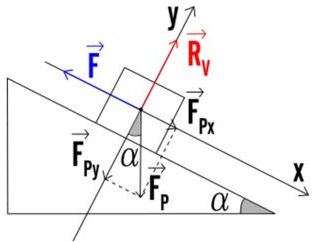
\includegraphics[width=0.4\linewidth]{Immagini/piano inclinato.png}
    \caption{diagramma delle forze di un piano inclinato.}
    \label{fig: piano inclinato}
\end{figure}
Riassumendo, se il corpo è fermo sul piano inclinato esso resta fermo per tutti gli angoli di inclinazione compresi tra zero e $\theta_s$ tale che $\tan{\theta_s}=\mu_{s}$; per $\theta>\theta_s$ il corpo non può restare fermo e scende lungo il piano inclinato. Però, una volta in moto, poiché $\mu_{d}<\mu_{s}$, si può avere moto anche per angoli minori di $\theta_s$, precisamente compresi tra $\theta_s$ e $\theta_d<\theta_s$ tale che $\tan{\theta_d}=\mu_{d}$.

Se invece il corpo all'istante iniziale sta scendendo lungo il piano con velocità $v_0$, esso si ferma se $mg\sin{\theta}<\mu_{d}mg\cos{\theta}$, cioè se $\tan{\theta}<\mu_{d}$, mentre si muove di moto uniformemente accelerato se $\tan{\theta}>\mu_{d}$ e prosegue con velocità $v_0$ se $\tan{\theta}=\mu_{d}$. L'unica differenza rispetto alla partenza da fermo è che si può avere moto anche se $\tan{\theta}<\mu_{d}$ proprio perché c'è una velocità iniziale.

\section{Forza elastica}
La forza elastica (unidimensionale) è una forza di direzione costante con verso rivolto sempre verso la posizione di equilibrio e con modulo proporzionale alla distanza da esso. Pertanto, la forza elastica è data da
\begin{equation}
    \vF_e=-k\vx.
\end{equation}
Dal secondo principio di Newton si ha che l'accelerazione vale
\begin{equation}
    a=-\frac{k}{m}x=-\omega^2x.
\end{equation}
Quindi il moto è armonico semplice con pulsazione $\omega$ e periodo
\begin{equation}
    T=\frac{2\pi}{\omega}=2\pi\sqrt{\frac{m}{k}}.
\end{equation}
Per verificarlo, si parte dal secondo principio di Newton $ma=-kx$ e si riscrive come
\begin{equation}
        \frac{d^2x}{dt^2}+\frac{k}{m}x=0,
\end{equation}
la quale non è altro che l'equazione dell'oscillatore armonico con soluzione
\begin{equation}
    x(t)=A\sin{(\omega t+\phi)}.
\end{equation}
I valori delle costanti $A$ e $\phi$ si ricavano dalle condizioni iniziali
\begin{equation}
    x_0=A\sin{\phi},\quad 0=\omega A\cos{\phi},
\end{equation}
dato che $v(t)=A\omega\cos{(\omega t+\phi)}$. Per $\phi\in(0,2\pi)$ sono possibili due soluzioni: $A=x_0$ per $\phi=\pi/2$ e $A=-x_0$ per $\phi=3\pi/2$; in ogni caso si hanno
\begin{equation}
    x(t)=x_0\cos{(\omega t)},\quad v(t)=-x_0\omega\sin{(\omega t)}.
\end{equation}
Se le condizioni iniziali sono diverse si ottiene sempre un moto armonico con la medesima $\omega$, però il valore dell'ampiezza è in generale diverso da $x_0$. Per esempio, con $x=x_0$ e $v=v_0$ per $t=0$, si ottiene
\begin{equation}
    A=\sqrt{x_0^2+\frac{v_0^2}{\omega^2}},\quad\tan{\phi}=\omega\frac{x_0}{v_0}.
\end{equation}
L'ampiezza $A$ è maggiore di $x_0$ a causa della velocità iniziale diversa da zero. Se in fatti si pone $v_0=0$ si ritrova il risultato precedente. 

\subsection{Tensione dei fili}
Si consideri un elemento infinitesimo $ds$ di un filo teso in quiete. Tale è ``tirato'' dalle due parti restanti di filo e l'equilibrio statico richiede che le due forze agenti sull'elemento di filo siano uguali in modulo e direzione, ma verso opposto.  Questo vale per ogni elemento di filo e il valore della tensione è lo stesso ovunque, altrimenti non ci sarebbe equilibrio. In particolare, ad un estremo $\vT=-\vF$. Per il filo $\overline{AB}$ nel suo insieme deve valere $F_A=F_B=T$: per tendere il filo si applicano le forze $\vF$ e $-\vF$ e la tensione, in modulo, è uguale al modulo di $\vF$. 

Si consideri ora un filo teso in movimento. L'ipotesi che il filo sia inestensibile comporta che tutti i punti del filo, compresi gli estremi, abbiano la stessa accelerazione. Pertanto, due corpi in movimento collegati da un filo teso devono avere la stessa accelerazione. L'ipotesi che il filo abbia massa trascurabile fa sì che il prodotto $ma$ risulti nullo per il filo e per qualsiasi suo elemento, quindi il valore della tensione durante il moto è lo stesso in qualunque punto del filo, come nel caso statico. Lo stesso succede, ovviamente, se il moto è uniforme; in tal caso $a=0$. 

Riassumendo, il filo teso esercita agli estremi la tensione $\vT$, il cui valore dipende dalle forze applicate e che deve essere pensata come la reazione del filo alla forza che lo tende. 

\subsubsection{Due corpi connessi da un filo}
Si considerino due corpi di massa $m_1$ e $m_2$ connessi da un filo di massa $m_f$ posti su un piano orizzontale. Si supponga l'azione di una forza $\vF$ sul corpo di massa $m_2$. 

In questa situazione, studiando il bilancio delle forze per i due corpi e il filo si ottengono
\begin{equation}
    \begin{cases}
        F-T_2=m_2a \\
        T_2-T_1=m_fa \\
        T_1=m_1a
    \end{cases}.
\end{equation}
Quindi, sostituendo la terza equazione nella seconda si ottiene
\begin{equation}
    T_2=(m_1+m_2)a.
\end{equation}
Sostituendo questa nella prima equazione si trova che la forza $F$ vale
\begin{equation}
    F=(m_1+m_2+m_f)a.
\end{equation}
Risolvendo per l'accelerazione e sostituendola nell'espressione delle due tensioni si ottengono
\begin{equation}
    T_1=\frac{m_1}{\sum_im_i},\quad T_2=\frac{m_f+m_1}{\sum_im_i},\quad i=1,2,f.
\end{equation}
\begin{obs}
    Se il filo è ideale, ossia se $m_f=0$, si ha $T_1=T_2$.
\end{obs}

\subsubsection{Pendolo semplice}
Si consideri un pendolo composto da una massa $m$ 
appesa ad un'estremità di un filo ideale di lunghezza $T$. La posizione di equilibrio statico è quella verticale, con la massa ferma e il filo teso. Se si inizia a spostare la massa di un certo angolo $\theta$ rispetto alla verticale, questa comincia ad oscillare intorno alla posizione di equilibrio. Le forze agenti su $m$ sono la forza peso $\vF=m\vg$ e la tensione del filo $\vT$, per cui il moto è regolato da $m\vg+\vT=\va$.
\begin{figure}[h]
    \centering
    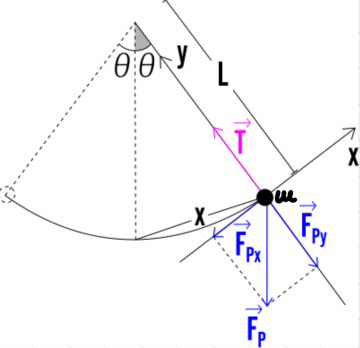
\includegraphics[width=0.4\linewidth]{Immagini/pendolo semplice.png}
    \caption{diagramma delle forze del pendolo semplice.}
    \label{fig: pendolo semplice}
\end{figure}

Scegliendo un sistema di riferimento adeguato, come quello in figura \ref{fig: pendolo semplice}, si può scomporre la forza peso nelle sue componenti
\begin{equation}
    F_x=-mg\sin{\theta},\quad F_y=mg\cos{\theta}.
\end{equation}
\begin{obs}
    Il segno negativo di $F_x$ è dovuto al fatto che la componente tangenziale della forza peso si oppone al moto della massa e tende sempre a riportarla alla posizione di equilibrio. Forze di questo genere sono dette forze di richiamo.
\end{obs}
Quindi, il bilancio delle forze sui due assi è
\begin{equation}
    \begin{cases}
        T-mg\cos{\theta}=ma_c=m\dfrac{v^2}{L} \\
        -mg\sin{\theta}=ma_T
    \end{cases}.
\end{equation}
Dalla seconda equazione si ricava l'equazione differenziale del moto del pendolo
\begin{equation}
    \frac{d^2\theta}{dt^2}+\frac{g}{L}\sin{\theta}=0.
\end{equation}
Tuttavia, per qualunque $\theta$ la soluzione è analiticamente complessa. Per semplificare il problema, si considerano angoli piccoli e si espande il seno in serie di Taylor 
\begin{equation}
    \sin{\theta}=\theta-\frac{\theta}{3!}+\cdots.
\end{equation}
Quantitativamente, per $\theta\le\SI{7}{\degree}$ si può approssimare $\sin{\theta}\simeq\theta$. Quindi, per piccole oscillazioni, l'equazione differenziale si riduce a
\begin{equation}
    \frac{d^2\theta}{dt^2}+\frac{g}{L}\theta=0,
\end{equation}
e coincide con quella del moto armonico semplice, ponendo $\omega^2=g/L$. Dunque, il moto del pendolo è oscillatorio armonico quando l'ampiezza delle oscillazioni è tale da poter approssimare $\sin{\theta}\simeq\theta$. La legge oraria del moto è
\begin{equation}
    \theta(t)=\theta_0\sin{(\omega t+\phi)},
\end{equation}
dove $\theta_0$ è l'ampiezza dell'oscillazione e $\phi$ è la fase iniziale, le quali dipendono dalle condizioni iniziali. Il periodo del moto è
\begin{equation}
    T=2\pi\sqrt{\frac{L}{g}},
\end{equation}
che è indipendente dall'ampiezza (isocronia delle piccole oscillazioni). La legge oraria dello spostamento lungo l'arco di circonferenza $s$ è
\begin{equation}
    s(t)=L\theta(t)=L\theta_0\sin{(\omega t+\phi)}.
\end{equation}
La velocità angolare $\omega(t)$ e la velocità lineare $v(t)$ hanno espressioni
\begin{equation}
    \omega(t)=\frac{d\theta}{dt}=\omega\theta_0\cos{(\omega t+\phi)},\quad v(t)=\frac{ds}{dt}=L\omega\theta_0\cos{(\omega t+\phi)}.
\end{equation}
Note $\theta(t)$ e $v(t)$, si può tornare all'equazione delle forze agenti lungo l'asse $y$ e trovare la tensione del filo
\begin{equation}
    T=m\bigg[g\cos{\theta(t)}+\frac{v^2(t)}{L}\bigg].
\end{equation}

\section{Lavoro, potenza ed energia cinetica}
Si è visto come il secondo principio di Newton si possa esprimere in termini di integrali attraverso il teorema dell'impulso, rivelando che si può calcolare una variazione finita della quantità di moto solo se si è capaci di calcolare l'integrale $\int_{t_0}^{t_1}F(t)\,dt$. Ora si estende il ragionamento considerando la forza come funzione della posizione occupata dal corpo. 

Si consideri un corpo puntiforme $P$ soggetto ad una forza $\vF$ che subisce uno spostamento $\Delta s$. Il lavoro $W$ compiuto dalla forza per lo spostamento $\Delta s$ è definito come il prodotto scalare della forza per lo spostamento, ovvero
\begin{equation}
\label{eq: definizione lavoro}
    W=\vF\cdot\Delta s=F\Delta s\cos{\theta}=F_T\Delta s,
\end{equation}
dove $\theta$ è l'angolo tra $\vF$ e $\Delta s$ e $F_T$ è la proiezione di $\vF$ lungo la direzione dello spostamento. Si possono presentare tre casi:
\begin{enumerate}
    \item Se $\theta<\pi/2$, allora l'accelerazione tangente è concorde con la velocità e la fa aumentare, quindi il lavoro risulta positivo e prende il nome di lavoro motore.
    \item Se  $\theta>\pi/2$, allora l'accelerazione tangente è discorde con la velocità e la fa diminuire, quindi il lavoro risulta positivo e prende il nome di lavoro resistente.
    \item Se $\theta=\pi/2$, allora la forza è ortogonale allo spostamento e il lavoro è nullo, in tal caso la forza è puramente centripeta e non fa variare il modulo della velocità.
\end{enumerate}
Per uno spostamento finito dal punto $A$ al punto $B$ lungo un percorso $C$, il lavoro si ottiene suddividendo tale percorso in una serie di $n$ segmenti $\Delta s_i$ e calcolando per ognuno di essi il lavoro $W_i=\vF_i\cdot\Delta s_i$. Sommando tutti i contributi si ottiene il lavoro totale $W=\sum_iW_i=\sum_i(\vF_i\cdot\Delta s_i)$. Questa è solo un'approssimazione del lavoro reale associato allo spostamento effettivo $C$, ma aumentando il numero di segmenti $n$ questa diventa sempre più accurata. Passando al limite $n\to\infty$, ogni segmento $\Delta s_i$ si confonde con lo spostamento infinitesimo $d\vs$ tangente in ogni punto a $C$, dunque il lavoro totale diventa
\begin{equation}
\label{eq: definizione lavoro spostamento finito}
    W=\int_A^B\vF\cdot d\vs=\int_A^BF\cos{\theta}\,ds.
\end{equation}
In altre parole, il lavoro è l'integrale di linea della forza.

Quando $\vF$ è la somma di $n$ forze $\vF_i$, per ciascuna si può calcolare il corrispondente lavoro e risulta
\begin{equation}
    \begin{split}
        W&=\int_A^B\vF\cdot d\vs=\int_A^B(\vF_1+\cdots+\vF_n)\cdot d\vs \\
        &=\int_A^B\vF_1\cdot d\vs+\cdots+\int_A^B\vF_n\cdot d\vs=W_1+\cdots+W_n.
    \end{split}
\end{equation}
Dunque, il lavoro è pari alla somma dei lavori delle singole forze agenti, ciascuno dei quali può essere positivo, negativo o nullo. 
\begin{defn}[potenza istantanea]
    Si definisce la potenza istantanea $P$ come il lavoro per unità di tempo
    \begin{equation}
        P=\frac{dW}{dt}=\vF\cdot\frac{d\vr}{dt}=\vF\cdot\vv=Fv\cos{\theta}.
    \end{equation}
\end{defn}
In generale, la potenza istantanea è variabile durante il moto e caratterizza la rapidità di erogazione del lavoro. Invece, la potenza media è il rapporto $W/\Delta t$, ossia è il rapporto tra il lavoro totale e l'intervallo di tempo in cui tale lavoro è stato svolto. Questa grandezza è fondamentale per descrivere le prestazioni di una macchina: a parità di lavoro totale svolto, ha maggiore potenza quella che lo eroga nel minor tempo. L'espressione del lavoro può essere scritta in forma infinitesima ottenendo
\begin{equation}
    dW=F_Tds=ma_T\,ds=m\frac{dv}{dt}\,ds=m\frac{ds}{dt}\,dv=mv\,dv.
\end{equation}
Si è trovato il legame esplicito tra il lavoro infinitesimo e la variazione infinitesima del modulo della velocità. Per un percorso finito dal punto $A$ al punto $B$ il lavoro vale
\begin{equation}
    W=\int_A^Bmv\,dv=\frac{1}{2}m(v_B^2-v_A^2)=K_B-K_A=\Delta K,
\end{equation}
dove la quantità $K=mv^2/2$ prende il nome di energia cinetica. Questo è il contenuto del teorema dell'energia cinetica.
\begin{teo}[teorema dell'energia cinetica]
    Qualunque sia la forza che agisce nello spostamento di un corpo puntiforme dal punto $A$ al punto $B$, il lavoro svolto dalla forza è uguale alla variazione dell'energia cinetica del corpo stesso.
\end{teo}

\subsection{Lavoro della forza peso}
Si calcola ora il lavoro della forza peso per uno spostamento generico dal punto $A$ al punto $B$. L'asse $z$ è orientato dal basso verso l'alto ed ha quindi verso opposto alla forza peso. Quindi, da \eqref{eq: definizione lavoro spostamento finito} si ha
\begin{equation}
    W=-mg\int_A^B\hatu_z\cdot d\vs=-mg\int_A^Bdz=-mg(z_B-z_A),
\end{equation}
dato che la forza peso ha come unica componente non nulla quella lungo l'asse $z$ e la componente di $\vr_{AB}$ lungo tale asse è $(z_B-z_A)$. Questo lavoro, dato che dipende unicamente dallo stato iniziale e finale, può essere scritto in termini di una funzione di stato $U(z)$. Dunque,
\begin{equation}
    W=-mg(z_B-z_A)=-[U(z_B)-U(z_A)]=-\Delta U(z)_{AB},
\end{equation}
dove $U(z)$ prende il nome di energia potenziale gravitazionale. 
\newpage
\noindent
Si presentano due casi:
\begin{enumerate}
    \item Se $z_A>z_B$, allora il lavoro svolto è positivo e per far avvenire lo spostamento è sufficiente la sola forza peso.
    \item Se $z_A<z_B$, allora il lavoro svolto è negativo e per fa avvenire lo spostamento è necessaria una forza esterna il cui lavoro superi quello resistente della forza peso oppure che abbia una velocità iniziale tale che la diminuzione di energia cinetica eguagli il lavoro.
\end{enumerate}

\subsection{Lavoro della forza elastica}
Il lavoro della forza elastica (unidimensionale) $\vF=-kx\hatu_x$ per uno spostamento finito lungo l'asse $x$ vale
\begin{equation}
    W=-k\int_A^Bx\hatu_x\cdot d\vs=-k\int_A^Bx\,dx=-\frac{1}{2}k(x_B^2-x_A^2).
\end{equation}
Come per la forza peso, dato che che dipende unicamente dallo stato iniziale e finale, può essere scritto in termini di una funzione di stato $U(x)$. Dunque, 
\begin{equation}
    W=-\frac{1}{2}k(x_B^2-x_A^2)=-[U(x_B)-U(x_A)]=-\Delta U(x)_{AB},
\end{equation}
dove $U(x)$ prende il nome di energia potenziale elastica. I casi che si presentano sono analoghi a quanto detto per la forza peso. 

\subsection{Lavoro della forza d'attrito radente}
Il lavoro della forza di attrito radente $\vF_{att}=-\mu_dN\hatu_s$, dove $\hatu_s$ è parallelo allo spostamento, vale
\begin{equation}
    W=\int_A^B-\mu_dN\hatu_s\cdot d\vs=-\mu_dN\int_A^Bds.
\end{equation}
L'integrale $\int_A^Bds$ non è altro che la lunghezza del percorso da $A$ e $B$ misurata lungo la traiettoria effettiva del corpo puntiforme. Pertanto, per la forza di attrito radente il lavoro dipende dal percorso seguito dal corpo e non è esprimibile in termini di una funzione di stato. Inoltre, il lavoro della forza di attrito è sempre negativo: se cambia il verso del moto, cambia anche quello della forza. Perché il moto possa avvenire o deve agire una forza che produca un lavoro superiore a quello di attrito o il corpo deve possedere una certa energia cinetica iniziale. L'energia cinetica diminuisce lungo il percorso e in $B$ la velocità è minore che in $A$. 

\section{Forze conservative}
Le forze per cui il lavoro non dipende dal percorso prendono il nome di forze conservative. Per il calcolo del lavoro si può considerare qualsiasi percorso che colleghi $A$ e $B$. Il lavoro è pertanto esprimibile in termini dei valori che una funzione di stato agli estremi $A$ e $B$. Questo implica che se si inverte il senso di percorrenza cambia solo il segno del lavoro
\begin{equation}
    \int_A^B\vF\cdot d\vs=-\int_A^B\vF\cdot d\vs.
\end{equation}
Per un percorso chiuso $ABA$ lungo la traiettoria $I$ e $-II$ percorsa in senso inverso si ha
\begin{equation}
    \int_A^B(\vF\cdot d\vs)_I+\int_A^B(\vF\cdot d\vs)_{-II}=\int_A^B(\vF\cdot d\vs)_I-\int_A^B(\vF\cdot d\vs)_{II}=0.
\end{equation}
Dunque, il lavoro svolto da una forza conservativa lungo qualsiasi percorso chiuso è nullo, ovvero
\begin{equation}
    \oint_\gamma\vF\cdot d\vs=0,\quad\forall\gamma.
\end{equation}
Riassumendo:
\begin{enumerate}
    \item per tutte le forze conservative il lavoro esprimere sempre come l'opposto della variazione o dell'energia potenziale relativa alla specifica forza
    \begin{equation}
        W=-\Delta U;
    \end{equation}
    \item non esiste una formula generale dell'energia potenziale, ma l'espressione esplicita dipende dalla particolare forza conservativa associata;
    \item nei casi della forza peso e della forza elastica l'energia potenziale è
    \begin{equation}
        U_p(z)=mgz,\quad U_e(x)=\frac{kx^2}{2}.
    \end{equation}
\end{enumerate}
\begin{obs}
    La relazione $W=\Delta K$ vale per qualsiasi forza agente, non solo per le forze conservative, a differenza di $W=-\Delta U$.
\end{obs}
Se agiscono solo conservative valgono sia $W=-\Delta U$ che $W=\Delta K$, quindi eguagliando le relazioni si ha
\begin{equation}
    U_A+K_A=U_B+K_B,
\end{equation}
ovvero la somma dell'energia cinetica e dell'energia potenziale di un corpo puntiforme che si muove sotto l'azione di forze conservative resta costante durante il moto, ossia si conserva. Tale somma prende il nome di energia meccanica. Pertanto, l'equazione trovata esprime il principio di conservazione dell'energia meccanica 
\begin{axiom}[principio di conservazione dell'energia meccanica]
    In presenza di sole forze conservative, l'energia meccanica di un corpo puntiforme si conserva, ovvero
    \begin{equation}
        E=K+U=costante.
    \end{equation}
\end{axiom}
In generale, quando agiscono sia forze conservative che non conservative, il lavoro complessivo è dato dalla somma del lavoro delle forze conservative $W_C$ e quello delle forze non conservative $W_{NC}$. Quindi, esprimendo $W_C=-\Delta U$, si ha
\begin{equation}
    W_{NC}=\Delta K+\Delta U=(K_B+U_B)-(K_A-U_A)=E_B-E_A=\Delta E.
\end{equation}
Dunque, in presenza di forze non conservative l'energia meccanica non si conserva, bensì la sua variazione è uguale al lavoro svolto dalle forze non conservative. 
\begin{ex}
    Considerando la situazione mostrata in figura \ref{fig: doppio piano inclinato} e, supponendo che $\tan{\theta}>\mu_d$, si vuole determinare la velocità con la quale il corpo arriva al punto $O$. 
    \begin{figure}[h]
        \centering
        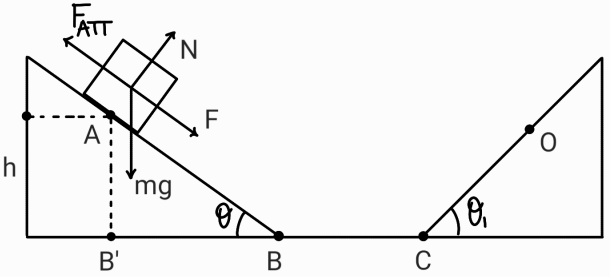
\includegraphics[width=0.57\linewidth]{Immagini/doppio piano inclinato.png}
        \caption{doppio piano inclinato in presenza di attrito.}
        \label{fig: doppio piano inclinato}
    \end{figure}
    
    Il lavoro della forza d'attrito lungo il tratto $\overline{PO}$ è
    \begin{equation}
        W_{att}=-\mu_dN|\overline{PO}|=-\mu_d(mg\cos{\theta})\frac{h}{\sin{\theta}}.
    \end{equation}
    Questo lavoro è uguale alla variazione di energia meccanica, quindi
    \begin{equation}
        -\mu_d(mg\cos{\theta})\frac{h}{\sin{\theta}}=\frac{mv_f^2}{2}-mgh,
    \end{equation}
    da cui si ricava la velocità finale 
    \begin{equation}
        v_f=\sqrt{2gh\bigg(1-\frac{\mu_d}{\tan{\theta}}\bigg)}.
    \end{equation}
\end{ex}
\begin{ex}
    Si consideri il moto di un pendolo semplice che parte dall'angolo di inversione $\theta_0$. Si assuma nulla l'energia potenziale nel punto più basso raggiunto dal pendolo (dove $P$ passa per la verticale). L'altezza di $P$, rispetto al livello zero, è $L(1-\cos{\theta})$. Le energie sono:
    \begin{enumerate}
        \item $U=mgL(1-\cos{\theta_0})$ e $K=0$ nel punto di inversione (il più alto raggiunto);
        \item $U=mgL(1-\cos\theta)$ e $K=mv^2/2$ in punto generico;
        \item $U=0$ e $K=mv_0^2/2$.
    \end{enumerate}
    Dal principio di conservazione dell'energia meccanica si ha
    \begin{equation}
        mgL(1-\cos{\theta})+mv^2/2=mgL(1-\cos{\theta_0}),
    \end{equation}
    da cui si ricava
    \begin{equation}
        v(\theta)=\sqrt{2gL(\cos{\theta}-\cos{\theta_0})}.
    \end{equation}
    In particolare, se $\theta=\pi/2$ si ha $v=\sqrt{2gL}$. Sostituendo $v(\theta)$ a $T-mg\cos{\theta}=mv^2/L$ si ha
    \begin{equation}
        T=mg(3\cos{\theta}-2\cos{\theta_0}),\quad\forall\theta_0.
    \end{equation}
\end{ex}
\begin{obs}
    La relazione integrale $-\Delta U=\int_A^B(F\hatu_x)\cdot d\vx$ può essere resa differenziale in $-dU=Fdx$, da cui si ricava
    \begin{equation}
        F=-\frac{dU}{dx}.
    \end{equation}
    Nel caso tridimensionale si hanno
    \begin{equation}
        F_x=-\frac{\p U}{\p x},\quad F_y=-\frac{\p U}{\p y},\quad F_z=-\frac{\p U}{\p z}.
    \end{equation}
    Usando la nozione di gradiente si ottiene
    \begin{equation}
        \vF=-\nabla U.
    \end{equation}
\end{obs}

\section{Momenti}
\begin{defn}[momento della forza]
    Si definisce il momento della forza come
    \begin{equation}
        \vM=\vr\times\vF.
    \end{equation}
\end{defn}
In generale, per calcolare un momento è necessario definire un polo $O$ rispetto a cui calcolarlo. Quindi, se il momento della forza rispetto al polo $O$ è $\vM=\bm{OP}\times\vF$ e la forza è applicata nel punto $P$, se si cambia polo in $O'$, allora il momento diventa
\begin{equation}
    \vM'=\bm{O'P}\times\vF.
\end{equation}
Dato che $\bm{O'P}=\bm{O'O}+\bm{OP}$, il momento $\vM'$ diventa
\begin{equation}
    \vM'=(\bm{O'O}+\bm{OP})\times\vF=\bm{O'O}\times\vF+\bm{OP}\times\vF=\bm{O'O}\times\vF+\vM.
\end{equation}
Quindi, in generale cambiando polo il momento della forza cambia anch'esso, e $\vM'=\vM$ se $\vF=m\va=0$ o se $\bm{O'O}\parallel\vF$.

Quando ad un punto sono applicate più forze con risultante $\vR=\sum_i\vF_i$, si ha
\begin{equation}
    \vM=\vr\times\vF_1+\cdots+\vr\times\vF_n=\vr\times(\vF_1+\cdots+\vF_n)=\vr\times\vR.
\end{equation}  
Quindi, il momento complessivo è uguale al momento della forza risultante. Pertanto, un sistema di forze applicate nello stesso punto può essere sempre sostituito, nel calcolo dell'accelerazione, del lavoro e del momento complessivo, dalla forza risultante. Questa proprietà non è valida se il punto di applicazione non è lo stesso per ogni forza.
\begin{defn}[momento angolare]
    Si definisce il momento angolare $\vL$ il momento del vettore quantità di moto, ovvero
    \begin{equation}
        \vL=\vr\times\vp=\vr\times m\vv.
    \end{equation}
\end{defn}
Analogamente al caso del momento della forza, se si cambia polo in $O'$, il momento angolare diventa
\begin{equation}
    \vL'=\bm{O'O}\times m\vv+\vL.
\end{equation}
\begin{obs}
    Dalla definizione di momento angolare, usando  $\vv=\vv_r+\vv_\theta$, questo si può riscrivere come
\begin{equation}
    \vL=\vr\times m(\vv_r+\vv_\theta)=m(\vr\times \vv_\theta),
\end{equation}
dove si è usato il fatto che $\vr\parallel\vv_r$ e $\vr\perp\vv_\theta$. Quindi
\begin{equation}
    L=mrv_\theta=mr(r\frac{d\theta}{dt})=mr^2\frac{d\theta}{dt}.
\end{equation}
\end{obs}
Dalla definizione di momento angolare si può ricavare un risultato importante. Derivando tale relazione si ha
\begin{equation}
\label{eq: derivata momento angolare}
    \frac{d\vL}{dt}=\frac{d\vr}{dt}\times m\vv+\vr\times m\frac{d\vv}{dt}.
\end{equation}
Ora si scelga un sistema di riferimento tale per cui il polo $O$ rispetto a cui si calcola il momento angolare sia fermo. Definendo $\vr$ come la distanza tra $O$ e la posizione del corpo puntiforme $P$, questa si può scrivere come $\vr=\vr_P-\vr_O$, dove $\vr_O$ e $\vr_P$  sono la distanza dall'origine del sistema di riferimento, rispettivamente, a $O$ e a $P$. Sostituendo la scomposizione di $\vr$ in \eqref{eq: derivata momento angolare} si ha
\begin{equation}
    \frac{d\vL}{dt}=\frac{d}{dt}(\vr_P-\vr_O)\times m\vv+\vr\times m\frac{d\vv}{dt},
\end{equation}
la quale, dato che $O$ è fermo rispetto al sistema di riferimento scelto, diventa
\begin{equation}
    \frac{d\vL}{dt}=\frac{d\vr_P}{dt}\times m\vv+\vr\times m\frac{d\vv}{dt},
\end{equation}
ma la derivata $d\vr_P/dt$ non è altro che la velocità $v$ del corpo puntiforme in $P$, che è la stessa per ogni sistema di riferimento inerziale, infatti $d\vr_P/dt=d\vr/dt$. Quindi, usando che $\vv\times \vv=0$, si ha
\begin{equation}
    \frac{d\vL}{dt}=\vr\times m\frac{d\vv}{dt}=r\times m\va=\vr\times\vF=\vM.
\end{equation}
Il risultato ottenuto costituisce il teorema del momento angolare.
\begin{teo}[teorema del momento angolare]
    La derivata temporale del momento angolare è uguale al momento della forza se entrambi i momenti sono riferiti allo stesso polo fisso in un sistema di riferimento inerziale, ovvero
    \begin{equation}
    \label{eq: relazione tra momento angolare e momento forze}
        \frac{d\vL}{dt}=\vM.
    \end{equation}
\end{teo}
Il momento della forza può essere nullo sia perché la forza applicata è nulla sia quando $\vr$ e $\vF$ sono paralleli. In questi casi si ha
\begin{equation}
    \frac{d\vL}{dt}=0\Rightarrow L=costante
\end{equation}
Dunque, se il momento delle forze è nullo, il momento angolare di un corpo puntiforme si conserva nel tempo. Integrando l'equazione \eqref{eq: relazione tra momento angolare e momento forze} si ha
\begin{equation}
    \int_0^t\vM\,dt=\Delta\vL.
\end{equation}
Quindi per produrre una variazione finita di momento angolare di un corpo puntiforme è necessaria l'azione, per un certo intervallo di tempo, di una forza. Questa proprietà è analoga al teorema dell'impulso. 
\begin{teo}[teorema del momento dell'impulso]
    Se la forza viene applicata per un intervallo di tempo molto breve, allora $\vr$ è praticamente costante e pertanto 
\begin{equation}
    \vr\times\vJ=\Delta \vL.
\end{equation}
In altre parole, la variazione di momento angolare è uguale al momento dell'impulso applicato.
\end{teo}
\begin{proof}
Dall'integrazione di \eqref{eq: relazione tra momento angolare e momento forze} si ha
    \begin{equation}
        \int_0^t\vM\,dt=\int_0^t\vr\times\vF\,dt=r\times\int_0^t\vF\,dt=\vr\times\vJ,
    \end{equation}
    ma dato che $\int_0^t\vM\,dt=\Delta L$, si trova $\vr\times\vJ=\Delta\vL$
\end{proof}
\begin{obs}
    Facendo riferimento al moto circolare, anche il lavoro può essere espresso in termini del modulo del momento della forza. Infatti
    \begin{equation}
        W=\int_A^B\vF\cdot d\vs=\int_{\theta_A}^{\theta_B}rF_T\,d\theta=\int_{\theta_A}^{\theta_B}M\,d\theta,
    \end{equation}
    dove si è usato il fatto che $ds=r\,d\theta$.
\end{obs}

\section{Forze centrali}
\begin{defn}[forza centrale]
    Una forza centrale è una qualsiasi forza che presenta le seguenti caratteristiche:
    \begin{enumerate}
        \item la direzione della forza deve passare per un punto fisso detto ``centro'';
        \item il modulo della forza deve dipendere esclusivamente dalla distanza dal centro.
    \end{enumerate}
\end{defn}
Un corpo puntiforme soggetto ad una forza centrale $\vF(\vr)$ può compiere una traiettoria qualsiasi, come mostrato in figura \ref{fig: forza centrale}. Per tale corpo, il momento angolare è conservato, infatti
\begin{equation}
    \vM=\vr\times\vF(\vr)=\vr\times(F\hatu_r)=F(\vr\times\hatu_r)=0,
\end{equation}
e pertanto $L=costante$. 
\begin{figure}[H]
    \centering
    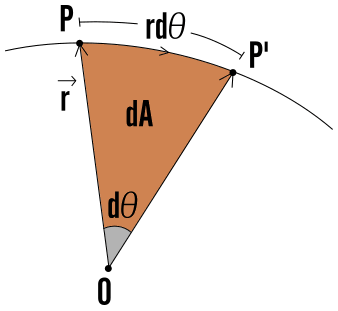
\includegraphics[width=0.4\linewidth]{Immagini/forze centrali.png}
    \caption{corpo puntiforme soggetto ad una forza centrale.}
    \label{fig: forza centrale}
\end{figure}

Quindi, in un intervallo di tempo $dt$, il vettore $\vr$ spazza un'area $dA$ approssimabile ad un triangolo di base $ds=r\,d\theta$ e di altezza $r$ (la differenza tra i lati e l'altezza è trascurabile), ossia
\begin{equation}
    dA=\frac{1}{2}r^2d\theta.
\end{equation}
Derivando rispetto al tempo questa relazione si ha
\begin{equation}
    \frac{dA}{dt}=\frac{1}{2}r^2\frac{d\theta}{dt}=\frac{L}{2m}=costante,
\end{equation}
dove si è usato che $L=mr^2(d\theta/dt)$. Il lavoro di una forza centrale è
\begin{equation}
    W=\int_A^B\vF(\vr)\cdot d\vs=\int_A^BF(r)\hatu_r\cdot d\vs=\int_A^BF(r)\,dr=F(r_B)-F(r_A),
\end{equation}
dove si è usato il fatto che $\hatu_r\cdot d\vs=\cos\theta\,d\vs=d\vr$. Dunque, dato che dipende unicamente dal valore della forza agli estremi, tutte le forze centrali sono conservative. 